\subsection*{Grey Box Sequence Diagram}
\begin{figure}[H]
	\centering
	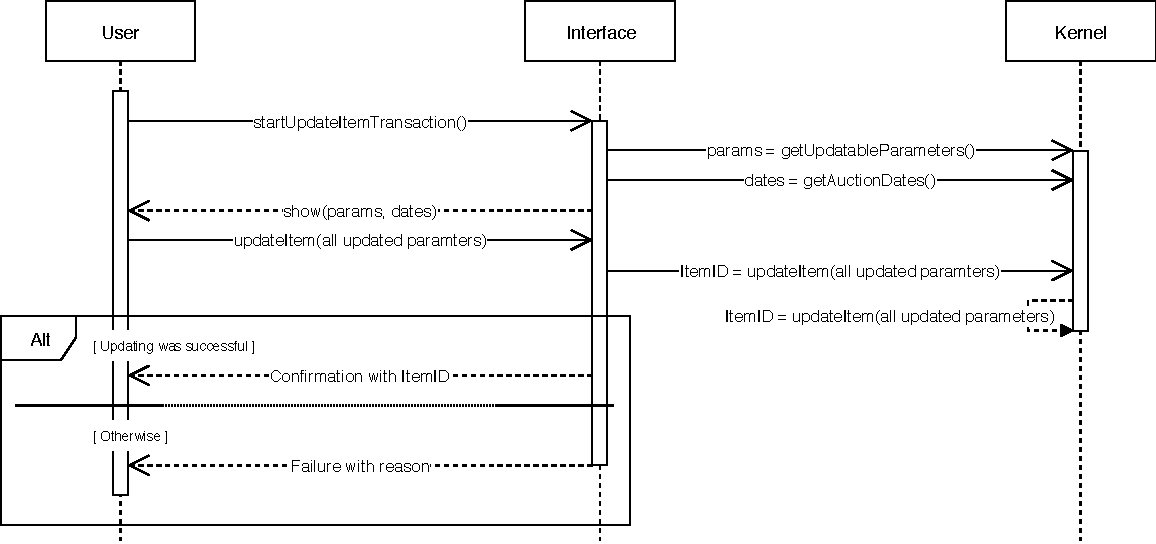
\includegraphics[scale=.9]{uml/SD-gb-update.pdf}
	\caption*{Grey Box diagram for use case B1, made by A}
\end{figure}
The interface in a grey box acts as an intermediate step between the actor and the kernel. User commands are passed to the interface, and it in turn can do some minor operations before delegating it to the kernel.\\For example, in this case, when the update item transaction is initiated, the interface responds by asking the kernel to get the updatable items, and passes them back to the actor. In essense, the interace is the translator between user/actor commands and kernel commands.
\subsection*{White Box Sequence Diagram}
\begin{figure}[H]
	\centering
	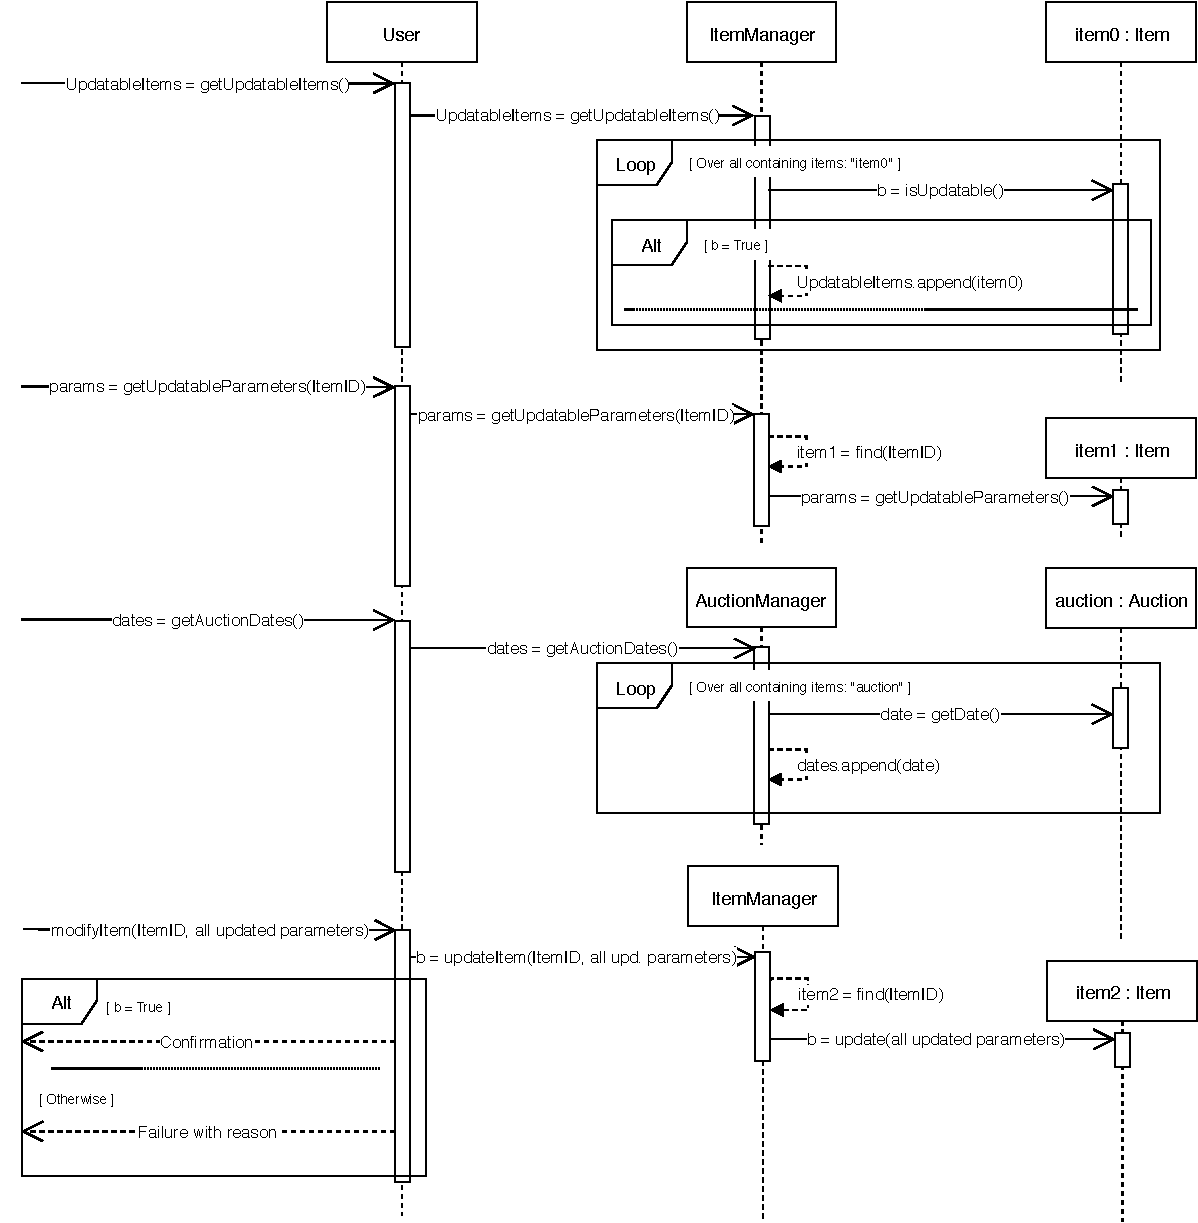
\includegraphics[scale=.85]{uml/SD-wb-update.pdf}
	\caption*{White Box diagram for use case B1, made by A}
\end{figure}
The white box is a high level implementation diagram for all kernel operations. The interface and actor are out of the picture, and everything is viewed from an implementation point of view.\\For example, the ``getUpdatableItems()'' function to the user class (found in the class diagram) is being delegated and executed in the ItemManager, which asks all individual items if they are updatable, and if so, appends them to a list which it returns.